% Created 2021-06-21 Mon 01:25
% Intended LaTeX compiler: pdflatex
\documentclass[11pt]{article}
\usepackage[utf8]{inputenc}
\usepackage[T1]{fontenc}
\usepackage{graphicx}
\usepackage{grffile}
\usepackage{longtable}
\usepackage{wrapfig}
\usepackage{rotating}
\usepackage[normalem]{ulem}
\usepackage{amsmath}
\usepackage{textcomp}
\usepackage{amssymb}
\usepackage{capt-of}
\usepackage{hyperref}
\usepackage[utf8x]{inputenc}
\usepackage[T2A]{fontenc}
\hypersetup{colorlinks, citecolor=black, filecolor=black, linkcolor=black, urlcolor=black}
\usepackage{pdfpages}
\author{q}
\date{\today}
\title{Матан. Подготвка к экзамену.}
\hypersetup{
 pdfauthor={q},
 pdftitle={Матан. Подготвка к экзамену.},
 pdfkeywords={},
 pdfsubject={},
 pdfcreator={Emacs 27.2 (Org mode 9.4.4)}, 
 pdflang={English}}
\begin{document}

\maketitle
\tableofcontents

\href{teory.pdf}{Pdf версия}

\section{Даты}
\label{sec:org8f18859}
\subsection{Консультация}
\label{sec:org2159bc7}
\emph{2021-06-24 Thu}
\subsection{Экзамен}
\label{sec:orgb87b71b}
\emph{2021-06-25 Fri}

\section{Видосы}
\label{sec:orgc9f7a63}
\subsection{Интегралы}
\label{sec:org4a6dfee}
\href{https://www.youtube.com/watch?v=nCx6FTChgow}{Интеграл: Азы интегрирования. Высшая математика}

\href{https://www.youtube.com/watch?v=wEmtlqJy2MM}{Определенный интеграл. Шпаргалка для первокурсника. Высшая математика}
\subsection{Ряды}
\label{sec:orgb023513}
\href{https://www.youtube.com/watch?v=XcofHzGx9Ug}{Математический анализ, 35 урок, Числовые ряды}

\href{https://www.youtube.com/watch?v=uq78fpEas5I}{Математический анализ, 36 урок, Достаточные признаки сходимости}
\section{Термины}
\label{sec:org7b61b67}
\subsection{{\bfseries\sffamily DONE} Бесконечно малая}
\label{sec:orgac98a99}
(также: бесконечно малая функция, бесконечно малая величина)

Функция \(\alpha(x)\) называется бесконечно малой при \(x\to a\), если \(\lim\limits_{x\to a}\alpha(x)=0\), т.е. для любого числа \(\varepsilon >0\) существует \(\delta>0\) такое, что из \(|x−a|<\delta\) следует \(|\alpha(x)|<\varepsilon\)

\subsection{{\bfseries\sffamily DONE} вертикальная асимптота}
\label{sec:org842223d}
Прямая \(x=a\) называется вертикальной асимптотой графика функции \(y=f(x)\), если хотя бы одно из предельных значений \(\lim\limits_{x\to a+0}f(x)\) или \(\lim\limits_{x\to a−0}f(x)\) равно \(+\infty\) или \(−\infty\).
\subsection{{\bfseries\sffamily DONE} возрастающая (убывающая) функция}
\label{sec:org7d1781f}
Говорят, что функция f(x) возрастает (убывает) на (a,b), если для любый точек x\textsubscript{1}<x\textsubscript{2} из (a,b) справедливо неравенство f(x\textsubscript{1})<f(x\textsubscript{2}) (f(x\textsubscript{1})>f(x\textsubscript{2}))
\subsection{{\bfseries\sffamily DONE} Второй замечательный предел}
\label{sec:org0b6496c}
 формула вида:
$$\lim\limits_{n\to \infty}(1+\frac{1}{n})^n=e$$
или
$$\lim\limits_{z\to 0}(1+z)^{\frac{1}{z}}=e$$

\subsection{{\bfseries\sffamily DONE} Дифференциал}
\label{sec:org49a5c91}
Если \(y=f(x)\) - дифференцируемая функция, то главная линейная чаcть \(A*\Delta x\) приращения функции f(x) называется дифференциалом функции и обозначается \(dy\).
\subsection{{\bfseries\sffamily DONE} Дифференцируемая функция}
\label{sec:org98f9401}
Функция \(y=f(x)\), определенная в некоторой окрестности точки \(x\). называтеся дифференцируемой в точке \(x\), если ее приращение в этой точке
$$\Delta y=f(x+\Delta x)−f(x)$$
имеет вид
$$\Delta y=A⋅\Delta x+\alpha(\Delta x)⋅\Delta x$$,
где \(A=const\), а функция \(\alpha(\Delta x)\to 0\) при \(\Delta x\to 0\).
\subsection{{\bfseries\sffamily DONE} евклидово пространство}
\label{sec:org7ee88f8}
Совокупность всех точек n-мерного пространства, в котором расстояние определяется по формуле
$$\rho(x,y)=\sqrt{(x_1−y_1)^2+…+(x_n−y_n)^2}$$,
называется n-мерным евклидовым пространством и обозначается \(R^n\).
\subsection{{\bfseries\sffamily DONE} координатная ось}
\label{sec:orgfdf877a}
Множество точек \(x=(x1,…,xn)\in R^n\) таких, что \(x_1=x_2=…=x_{i−1}=x_{i+1}=…=x_{n}=0\), называется \$i\$-й координатной осью \((i=1,…,n)\) этого пространства. Точка \(0=(0,…,0)\) называется началом координат.
\subsection{{\bfseries\sffamily DONE} Критическая точка}
\label{sec:org9b69cc0}
Точка \(x_0\) называется критической, если \(f'(x_0)=0\) или \(f'(x_0)\) не существует.
\subsection{{\bfseries\sffamily DONE} локальный максимум (минимум)}
\label{sec:org801f86c}
Говорят, что функция \(y=f(x)\) имеет (или достигает) в точке \(\alpha\) локальный максимум (минимум), если найдется такая окрестность \(U(\alpha)\) точки \(\alpha\), что для всех \(x\in U(\alpha)\):
$$f(\alpha)\geq f(x)$$ 
$$(f(a)\leq f(x))$$
Локальный минимум и локальный максимум объединяют общим названием - локальный экстремум.
\subsection{{\bfseries\sffamily DONE} наклонная асимптота}
\label{sec:org1de9b63}
Прямая \(y=kx+b\) называется наклонной асимпотой графика функции \(y=f(x)\) при \(x\to \infty\) \((-\infty)\), если
$$f(x)=kx+b+\alpha(x)$$
$$\lim\limits_{x\to\pm\infty}\alpha(x)=0$$
\subsection{{\bfseries\sffamily DONE} Неопределенный интеграл}
\label{sec:org54d9d77}
Неопределенным интегралом от данной функции f(x) называется множество всех его первообразных
$$\int f(x)dx=F(x)+C$$
$$F'(x)=f(x)$$.
\subsection{{\bfseries\sffamily DONE} непрерывная функция}
\label{sec:org6c6a471}
Функция называется непрерывной в точке x\textsubscript{0}, если бесконечно малому приращению \(\Delta x\) аргумента \(x\) в точке x\textsubscript{0} соответствует бесконечно малое приращение функции \(\Delta y\). т.е.
$$\lim\limits_{\Delta x\to 0}\Delta y=\lim\limits_{\Delta x\to 0}[f(x_0+\Delta x)−f(x_0)]=0$$
\subsection{{\bfseries\sffamily DONE} несобственный интеграл первого рода}
\label{sec:orgdaa0f88}
Сходящимся несобственным интегралом первого рода \(\int_{a}^{\infty}f(x)dx\) от функции \(f(x)\) в интервале \([a,\infty)\) называется предел:
$$\int_{a}^{\infty}f(x)dx=\lim\limits_{b→\infty}\int_{a}^{b}f(x)dx$$
\subsection{{\bfseries\sffamily DONE} неубывающая (невозрастающая) функция}
\label{sec:orgfb9a9eb}
Говорят, что функция \(f(x)\) не убывает (не возрастает) на \((a,b)\), если для любых точек x\textsubscript{1}<x\textsubscript{2} из \((a,b)\) справедливо неравенство
$$f(x_1)\leq f(x_2)$$
$$(f(x_1)\geq f(x_2))$$
\subsection{{\bfseries\sffamily DONE} неявная функция}
\label{sec:org227749e}
Неявная функция - это функция \(y(x)\) заданная некоторым уравнением \(F(x,y)=0\).
\subsection{{\bfseries\sffamily DONE} окрестность точки}
\label{sec:org956ffd1}
Пусть \(x\in R^n\), \(\varepsilon >0\). Совокупность всех точек \(y\in R^n\) таких, что \(\rho(x,y)<\varepsilon\), называется n-мерным шаром с центром в точке \(X\) радиуса \(\varepsilon\) или \(\varepsilon\)-окрестностью:

$$U(x;\varepsilon)=\{y: y\in R^n,\rho(x,y)<\varepsilon\}$$.
\subsection{{\bfseries\sffamily DONE} Определенный интеграл}
\label{sec:org3c817e2}
Определенным интегралом от функции f(x) на [a,b] называется предел интегральной суммы
$$\lim\limits_{n\to\infty}\Sigma_{i=1}^{n}f(\xi_i)\Delta x_i$$,
если он существует. Здесь \(\xi_i\in[x_{i−1},x_i]\) и \(a=x_0<x_1<…x_n=b\).

Обозначение интеграла:
 $$\int_{a}^{b}f(x)dx$$
\subsection{{\bfseries\sffamily DONE} Первообразная}
\label{sec:org2cd46fa}
Первообразной от функции \(f(x)\) в данном интервале называется функция \(F(x)\), производная которой равна данной функции:
$$F'(x)=f(x)$$
\subsection{{\bfseries\sffamily DONE} Первый замечательный предел}
\label{sec:orge6c4aa8}
$$\lim\limits_{x\to 0}\frac{\sin x}{x}=1$$
\subsection{{\bfseries\sffamily DONE} Предел функции}
\label{sec:org39ce68e}
(на языке \(\varepsilon\)-\(\delta\)) Число \(A\) называется пределом функции \(y=f(x)\) при \(x\to x_0\), если существует такое число \(\delta(\varepsilon)\), что для всех \(x\ne x_0\), удовлетворяющих условию \(|x−x_0|<\delta\) имеет место неравенство
$$|f(x)−A|<\varepsilon$$
\subsection{{\bfseries\sffamily DONE} производная функции}
\label{sec:orgef7b01c}
Производной функции \(y=f(x)\) в данной фиксированной точке x называется предел
$$\lim\limits_{\Delta x→0}\frac{f(x+\Delta x)−f(x)}{\Delta x}$$
если этот предел существует.
\subsection{{\bfseries\sffamily DONE} прямоугольная окрестность точки}
\label{sec:org25ebf05}
Прямоугольной окрестностью точки \(x=(x_1,…,x_n)\in R^n\) называется множество 
$$P(x;δ_1,…,δ_n)=\{(y_1,…,y_n):|x_i−y_i|<δ_i ,1\leq i\leq n\}, δ_i>0$$
\subsection{{\bfseries\sffamily DONE} разрыв второго рода}
\label{sec:orgb203fe9}
Точка a называется точкой разрыва второго рода, если в этой точке функция \(f(x)\) не имеет по крайней мере одного из односторонних пределов или хотя бы один из односторонних пределов бесконечен.
\subsection{{\bfseries\sffamily DONE} разрыв первого рода}
\label{sec:orgcfd509e}
Точка a называется точкой разрыва первого рода, если в этой точке \(f(x)\) имеет конечные, но не равные друг другу правый и левые пределы
$$\lim\limits_{x\to a+0}f(x)\ne\lim\limits_{x\to a−0}f(x)$$
\subsection{{\bfseries\sffamily DONE} расстояние между точками}
\label{sec:orgeb00158}
Расстояние между двумя точками \((x_1,…,x_n)\) и \((y_1,…,y_n)\) определяется по формуле:

$$\rho(x,y)=\sqrt{(x_1−y_1)^2+…+(x_n−y_n)^2}$$
\subsection{{\bfseries\sffamily DONE} сложнопоказательная функция}
\label{sec:org1e1740e}
Функция вида \(y=u(x)^{v(x)},(u(x)>0)\), где и основание, и показатель степени зависят от x, называется сложнопоказательной.
\subsection{{\bfseries\sffamily DONE} Стационарная точка}
\label{sec:org931beb5}
Точка \(x_0\) называется стационарной для функции \(f(x)\), если \(f(x)\) дифференцируема в точке \(x_0\) и \(f'(x_0)=0\).
\subsection{{\bfseries\sffamily DONE} точка пространства}
\label{sec:org0a32e5a}
Точкой x n-мерного пространства называется упорядоченная совокупность n действительных чисел \((x_1,…,x_n)=x\).
Число \(x_i\) называется i-й координатой точки \(x, i=1,…,n\).
\subsection{{\bfseries\sffamily DONE} устранимый разрыв}
\label{sec:org264b7ff}
Точка a называется точкой устранимого разрыва функции \(y=f(x)\), если предел функции \(f(x)\) в точке \emph{a} существует, но в самой точке \emph{a} значение \(f(x)\) либо не существует, либо не равно пределу \(f(x)\) в этой точке. 
\section{Темы}
\label{sec:orgfe9f467}
\subsection{{\bfseries\sffamily DONE} Все билеты, рукописный вариант}
\label{sec:org4f9a772}
\href{bilets/all.pdf}{all}

\subsection{{\bfseries\sffamily DONE} Билет 1}
\label{sec:org22c2775}
Первообразная и неопределенный интеграл (определения). Свойства интеграла. Таблица основных неопределенных интегралов. Формула замены переменной в неопределенном интеграле (с доказательством). Формула интегрирования по частям.
\subsubsection{{\bfseries\sffamily DONE} Опр. 1.}
\label{sec:org2287d82}
Функция \emph{F} называется первообразной функции \emph{f} на промежутке \(\Delta\) , если \emph{F} дифференцируема на \(\Delta\) и в каждой точке \emph{x} \(\in\) \(\Delta\)
\begin{eqnarray}
F'(x)=f(x)
\end{eqnarray}
Очевидно, что первообразная \emph{F(x)} непрерывна на \(\Delta\).

\subsubsection{{\bfseries\sffamily DONE} Опр. 2.}
\label{sec:orgd3999da}
Пусть функция \emph{f(x)} задана на промежутке \(\Delta\). Совокупность всех ее первообразных на этом промежутке называется \emph{\textbf{неопределенным интегралом от функции \emph{f}}} и обозначается

\begin{eqnarray}
\int f(x)dx
\end{eqnarray}

Если \emph{F(x)} — какая-либо первообразная функции \emph{f(x)} на \(\Delta\), то пишут

\begin{eqnarray}
\int f(x)dx=F(x)+C
\end{eqnarray}

\emph{C} — произвольная постоянная.

\subsubsection{{\bfseries\sffamily DONE} Основные свойства интеграла}
\label{sec:orgbe249d2}
\begin{enumerate}
\item Если функция \emph{F(x)} дифференцируема на \(\Delta\), то
\label{sec:org9d5fc55}

\begin{eqnarray}
\int dF(x)=F(x)+C \text{ или }\int F'(x)dx=F(x)+C
\end{eqnarray}

\item Пусть функция \emph{f(x)} имеет первообразную на \(\Delta\). Тогда для любого \emph{x} \(\in\) \(\Delta\) имеет место равенство:
\label{sec:orga0cafed}

\begin{eqnarray}
d\int f(x)=f(x)dx
\end{eqnarray}

\item Если функции \emph{f\textsubscript{1}}, \emph{f\textsubscript{2}} имеют первообразные на \(\Delta\), то функция \emph{f\textsubscript{1}} + \emph{f\textsubscript{2}} имеет первообразную на \(\Delta\), причем:
\label{sec:org92e988c}

\begin{eqnarray}
\int(f_1(x) + f_2(x))dx=\int f_1(x)dx + \int f_2(x)dx
\end{eqnarray}

\item Если функция \emph{f(x)} имеет первообразную на \(\Delta\), \emph{k} \(\in\) \emph{\R}, то функция \emph{kf(x)} также имеет на \(\Delta\) первообразную, и при \emph{k} \(\ne\) 0:
\label{sec:org95818f0}

\begin{gather*}
\int kf(x)dx=\{kF(x)+C\}\text{, }k\int f(x)dx=k\{F(x)+C\}
\end{gather*}

Т.к. \emph{C} – произвольная постоянная и \emph{k} \(\ne\) 0, то множества \({kF(x) + C}\) и \(k{F(x) + C}\) совпадают.
\end{enumerate}

\subsubsection{{\bfseries\sffamily DONE} След. 1 (Линейность интеграла)}
\label{sec:org23008c2}
Если f\textsubscript{1} и f\textsubscript{2} имеют первообразные на \(\Delta\), \(\lambda\)\textsubscript{1}, \(\lambda\)\textsubscript{2} \(\in\) \R, \(\lambda_1^2+\lambda_2^2>0\), 
то функция \(\lambda_1 f_1+\lambda_2 f_2\) имеет первообразную на \(\Delta\), причем

\begin{eqnarray}
\int(\lambda_1 f_1(x)+\lambda_2 f_2(x))dx=\lambda_1\int f_1(x)dx+\lambda_2\int f_2(x))dx
\end{eqnarray}

Доказательство вытекает из свойств 3 и 4.
\subsubsection{{\bfseries\sffamily DONE} Формула замены переменной}
\label{sec:org04bbc6c}
Пусть функции \(f(x)\) и \(\varphi(t)\) заданы соответственно на промежутках \(\Delta_x\) и \(\Delta_t\), 
причем \(\varphi (\Delta_t) = \Delta_x\), т.е. имеет смысл сложная функция \(f(\varphi(t))\), \(t \in \Delta_t\). 
Пусть, кроме того, функция \(\varphi(t)\) дифференцируема и строго монотонна на \(\Delta_t\). Тогда у функции \(\varphi(t)\)
существует обратная однозначная функция \(\varphi^{-1}(x)\), определенная на промежутке \(\Delta_x\).
\begin{enumerate}
\item \textbf{Теорема 1.}
\label{sec:orgd18de0e}
Существование на промежутке \(\Delta_x\) интеграла

  \begin{eqnarray}
\int f(x)dx
  \end{eqnarray}

и существование на промежутке \(\Delta_t\) интеграла

  \begin{eqnarray}
\int f(\varphi(t))\varphi'(t)dt
  \end{eqnarray}

равносильны, и имеет место формула

  \begin{eqnarray}
\int f(x)dx=\int f(\varphi(t))\varphi'(t)dt\bigg|_{t=\varphi^{-1}(x)}
  \end{eqnarray}

Формула (10) называется формулой замены переменной в неопределенном интеграле:
переменная x заменяется переменной t по формуле \(x = \varphi(t)\).
\item \textbf{Доказательство.}
\label{sec:org3bf0fa4}
Докажем, что существование первообразной у функции f(x) на
 \(\Delta\)\textsubscript{x} равносильно существованию первообразной у функции \(f(\varphi(t))\varphi'(t)\)  на \(\Delta\)\textsubscript{t}
 . Пусть у функции f(x) на \(\Delta\)\textsubscript{x} существует первообразная F(x), т.е.

\begin{eqnarray}
\frac{dF(x)}{dx} = f(x)\text{, } x\in\Delta_t
\end{eqnarray}

Имеет смысл сложная функция \(F(\varphi(t))\), она является первообразной функции \(f(\varphi(t))\varphi'(t)\) на \(\Delta\)\textsubscript{t}. 
Действительно,

\begin{eqnarray}
\frac{d}{dt}F(\varphi(t))=\frac{dF(x)}{dx}\bigg|_{x=\varphi(t)}*\frac{d\varphi(t)}{dt}=f(\varphi(t))\varphi'(t)
\end{eqnarray}

Обратно. Пусть функция \(f(\varphi(t))\varphi'(t)\) имеет первообразную \(\Phi\)(t), тогда

\begin{eqnarray}
 \frac{d\Phi(t)}{dt}=f(\varphi(t))\varphi'(t)
 \end{eqnarray}

Покажем, что  \(\Phi(\varphi^{-1}(x))\) является на \(\Delta\)\textsubscript{x} первообразной функции f(x). В самом
деле,

$$
 \frac{d}{dt}\Phi(\varphi^{-1}(x))=\frac{d\Phi(t)}{dt}\bigg|_{t=\varphi^{-1}(x)}*\frac{d\varphi^{-1}(x)}{dx}=
(f(\varphi(t))\varphi'(t))\bigg|_{t=\varphi^{-1}(x)}*\frac{d\varphi^{-1}(x)}{dx}=f(x).
$$

Итак, интегралы (8) и (9) одновременно существуют или нет. При этом

\begin{eqnarray}
 \int f(x)dx=F(x)+C
 \end{eqnarray}
$$
\int f(\varphi(t))\varphi'(t)dt=F(\varphi(t))+C
$$
 а так как \(F(\varphi(t))|_{t=\varphi^{-1}(x)}=F(x)\), имеет равенство (10).
\end{enumerate}
\subsubsection{{\bfseries\sffamily DONE} Формула интегрирования по частям}
\label{sec:orge1b7a90}
\begin{enumerate}
\item Теорема 2.
\label{sec:org81cf2aa}
Если функции \(u(x)\), \(v(x)\) дифференцируемы на некотором промежутке
\(\Delta\) и на этом промежутке существует \(\int vdu\), то на нем существует интеграл 
\(\int udv\), причем
\begin{eqnarray}
\int u(x)dv(x)=u(x)v(x)-\int v(x)du(x).
\end{eqnarray}
Формула (15) называется \textbf{\emph{формулой интегрирования по частям.}}
\item Доказательство.
\label{sec:orgb06381d}
Пусть \(u(x)\), \(v(x)\) — дифференцируемы на \(\Delta\), тогда

$$
d(u(x)v(x))=v(x)du(x)+u(x)dv(x)\Rightarrow u(x)dv(x)=d(u(x)v(x))-v(x)du(x).
$$

Проинтегрируем обе части полученного равенства:

$$
\int u(x)dv(x)=\int(d(u(x)v(x))-v(x)du(x))=u(x)v(x)-\int v(x)du(x).
$$
\end{enumerate}

\subsection{{\bfseries\sffamily TODO} Билет 2}
\label{sec:orgc316861}
Определенный интеграл Римана (определение). Ограниченность интегрируемых функций (с доказательством). Верхние и нижние суммы Дарбу (определения). Верхний и нижний интегралы Дарбу (определения). Критерий Дарбу. Интегрируемость непрерывных функций. Интегрируемость монотонных функций.

\subsubsection{{\bfseries\sffamily DONE} Опр 1.}
\label{sec:orgbe8f39c}
Множество точек \(\tau=\{x_k\}_{k=0}^{k=k_\tau}\) отрезка \([a,b]\subset \mathbb{R}\) таких, что

$$
a=x_0 < x_1 < ... < x_{k_\tau-1} < x_{k_\tau} = b
$$

называют \textbf{\emph{разбиением \(\tau\) отрезка}} [a, b]. 

Точки x\textsubscript{k} — точки разбиения \(\tau\) , отрезки [x\textsubscript{k-1}, x\textsubscript{k}]
 — отрезки разбиения \(\tau\) , \(\Delta x_k = x_k − x_{k-1}\) — их длины, \(|\tau | = \max \{\Delta x_1 ,... , \Delta x_{k_\tau}\}\) называют */мелкостью разбиения (или диаметром разбиения)*/.

Отметим два очевидных свойства разбиений:
\begin{enumerate}
\item Если \(\tau<\tau',\tau'<\tau''\), то \(\tau<\tau''\).
\item Для любых разбиений \(\tau', \tau''\) существует разбиение \(\tau : \tau < \tau', \tau < \tau''\).
\end{enumerate}
Пусть функция f определена на \([a, b], a < b, \tau = \{x_k\}_{k=0}^{k=k_\tau}\) — некоторое разбиение
этого отрезка. Всякая сумма \(\sigma_\tau\) вида
$$
\sigma_\tau = \sigma_\tau(f,\xi_1,...,\xi_{k_\tau})=\sum_{k=1}^{k_\tau}f(\xi_{k})\Delta x_k, \xi_k\in[x_{k-1},x_k]
$$
называется \textbf{\emph{интегральной суммой Римана}} функции f

\subsubsection{{\bfseries\sffamily DONE} Опр 2.}
\label{sec:org1202c3a}
Функция f называется \textbf{\emph{интегрируемой по Риману на отрезке}}
 \([a, b]\), если существует число \(I\) такое, что для любой последовательности разбиений
 \(\tau_n = \{x_k^n\}_{k=0}^{k=k_{\tau_n}}, n\in \mathbb{N}\), отрезка [a, b] диаметры которых стремятся к нулю при \$n\(\to\) \(\infty\) \((\lim\limits_{n\to\infty}|\tau_n|=0)\) и для любого набора точек
$$
\xi_k^n\in[x_{k-1}^n, x_k^n], k=1,2,...,k_{\tau_n}, n\to\mathbb{N}
$$
 существует предел интегральных сумм
$$
\lim\limits_{n\to\infty}\sigma_{\tau_n}(f,\xi_1^n,...,\xi_{k_{\tau_n}}^n) = I
$$
 Число \(I\) \textbf{\emph{называют интегралом Римана от функции f на отрезке}} [a, b] и обозначают \(\int_a^bf(x)dx\)

\subsection{{\bfseries\sffamily DONE} Билет 3}
\label{sec:org0fac541}
Свойства определенного интеграла (сформулировать все, доказать непрерывность интеграла по верхнему пределу). Интегральная теорема о среднем.
\href{bilets/3.pdf}{3}


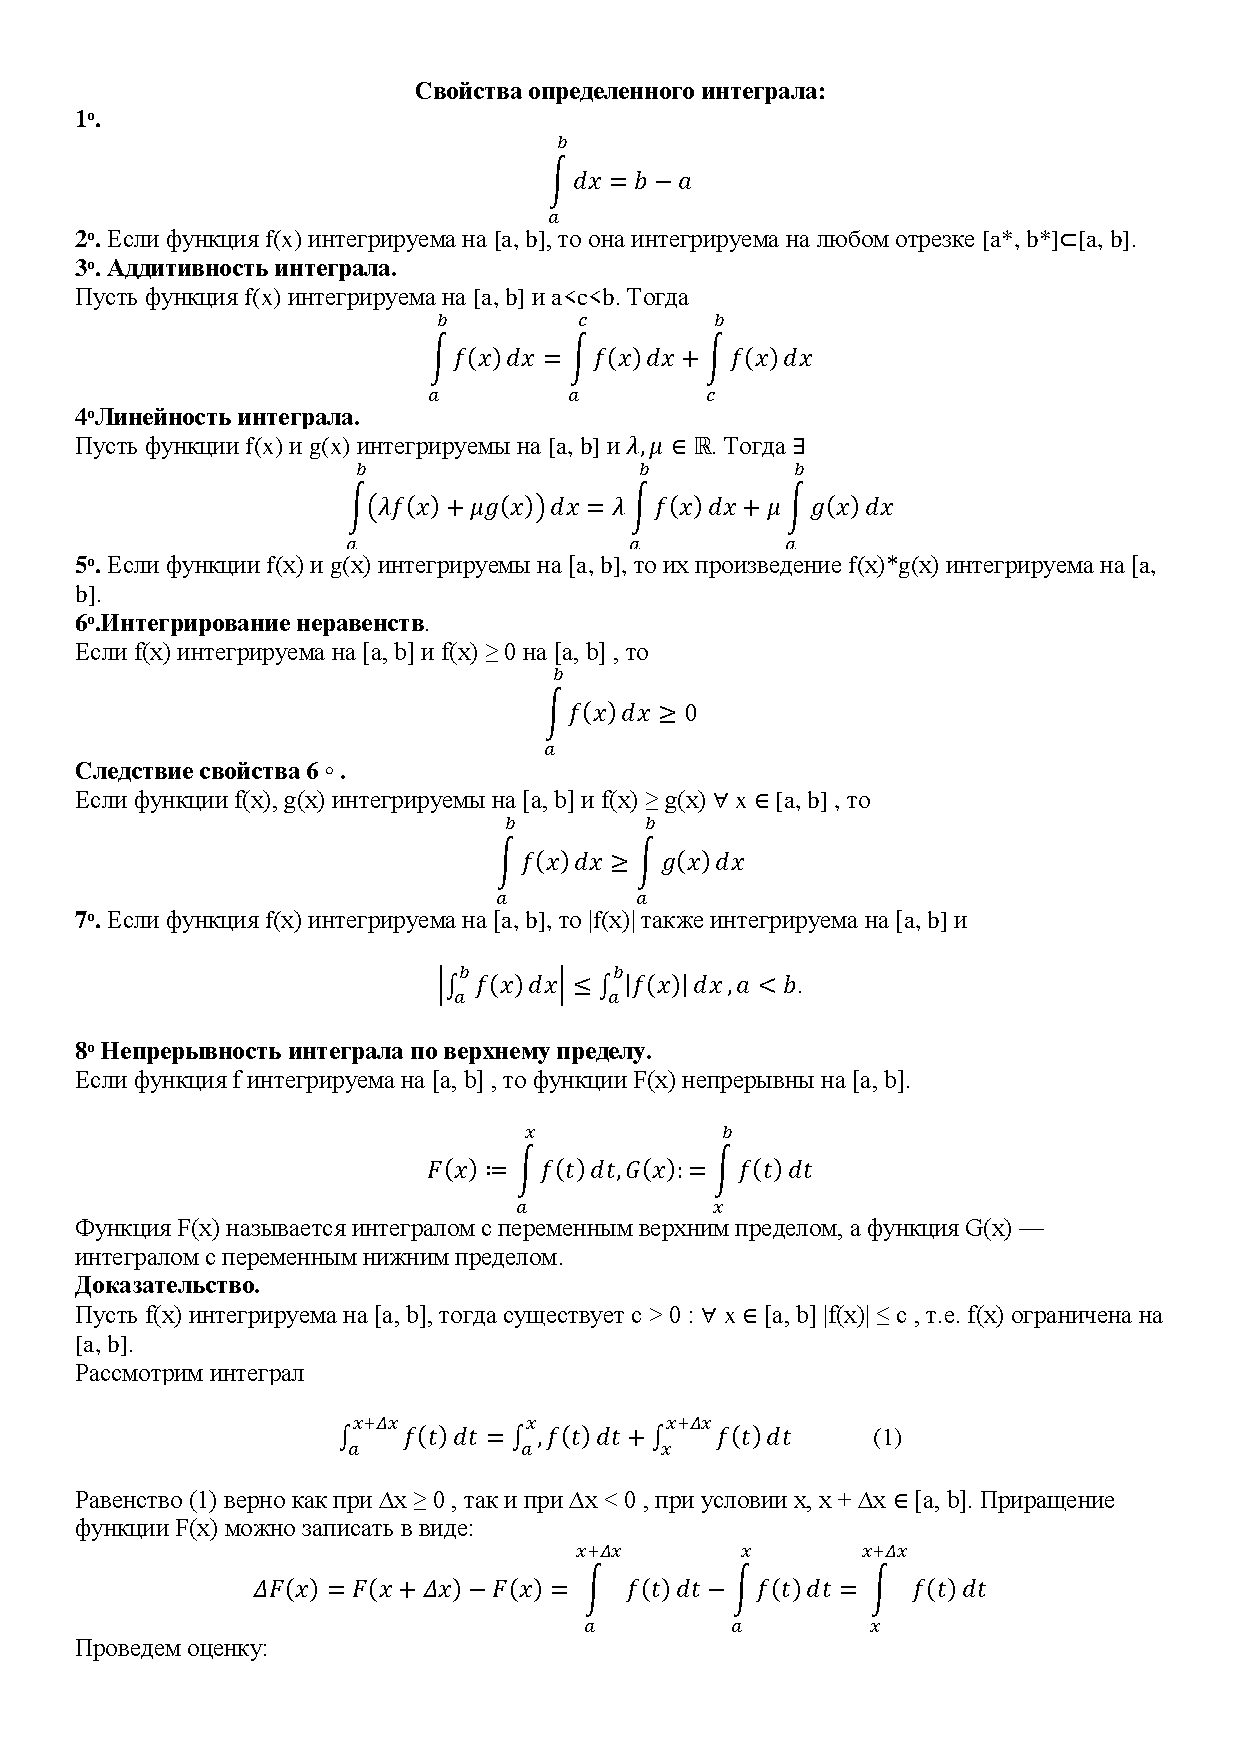
\includepdf[pages=-]{bilets/3.pdf}


\subsection{{\bfseries\sffamily DONE} Билет 4}
\label{sec:org13f9fc1}
Теорема о дифференцировании интеграла по верхнему пределу (с доказательством).  Теорема о существовании первообразной (с доказательством). Формула Ньютона-Лейбница (с доказательством). Формула замены переменной в определенном интеграле. Формула интегрирования по частям.
\href{bilets/4.pdf}{4}


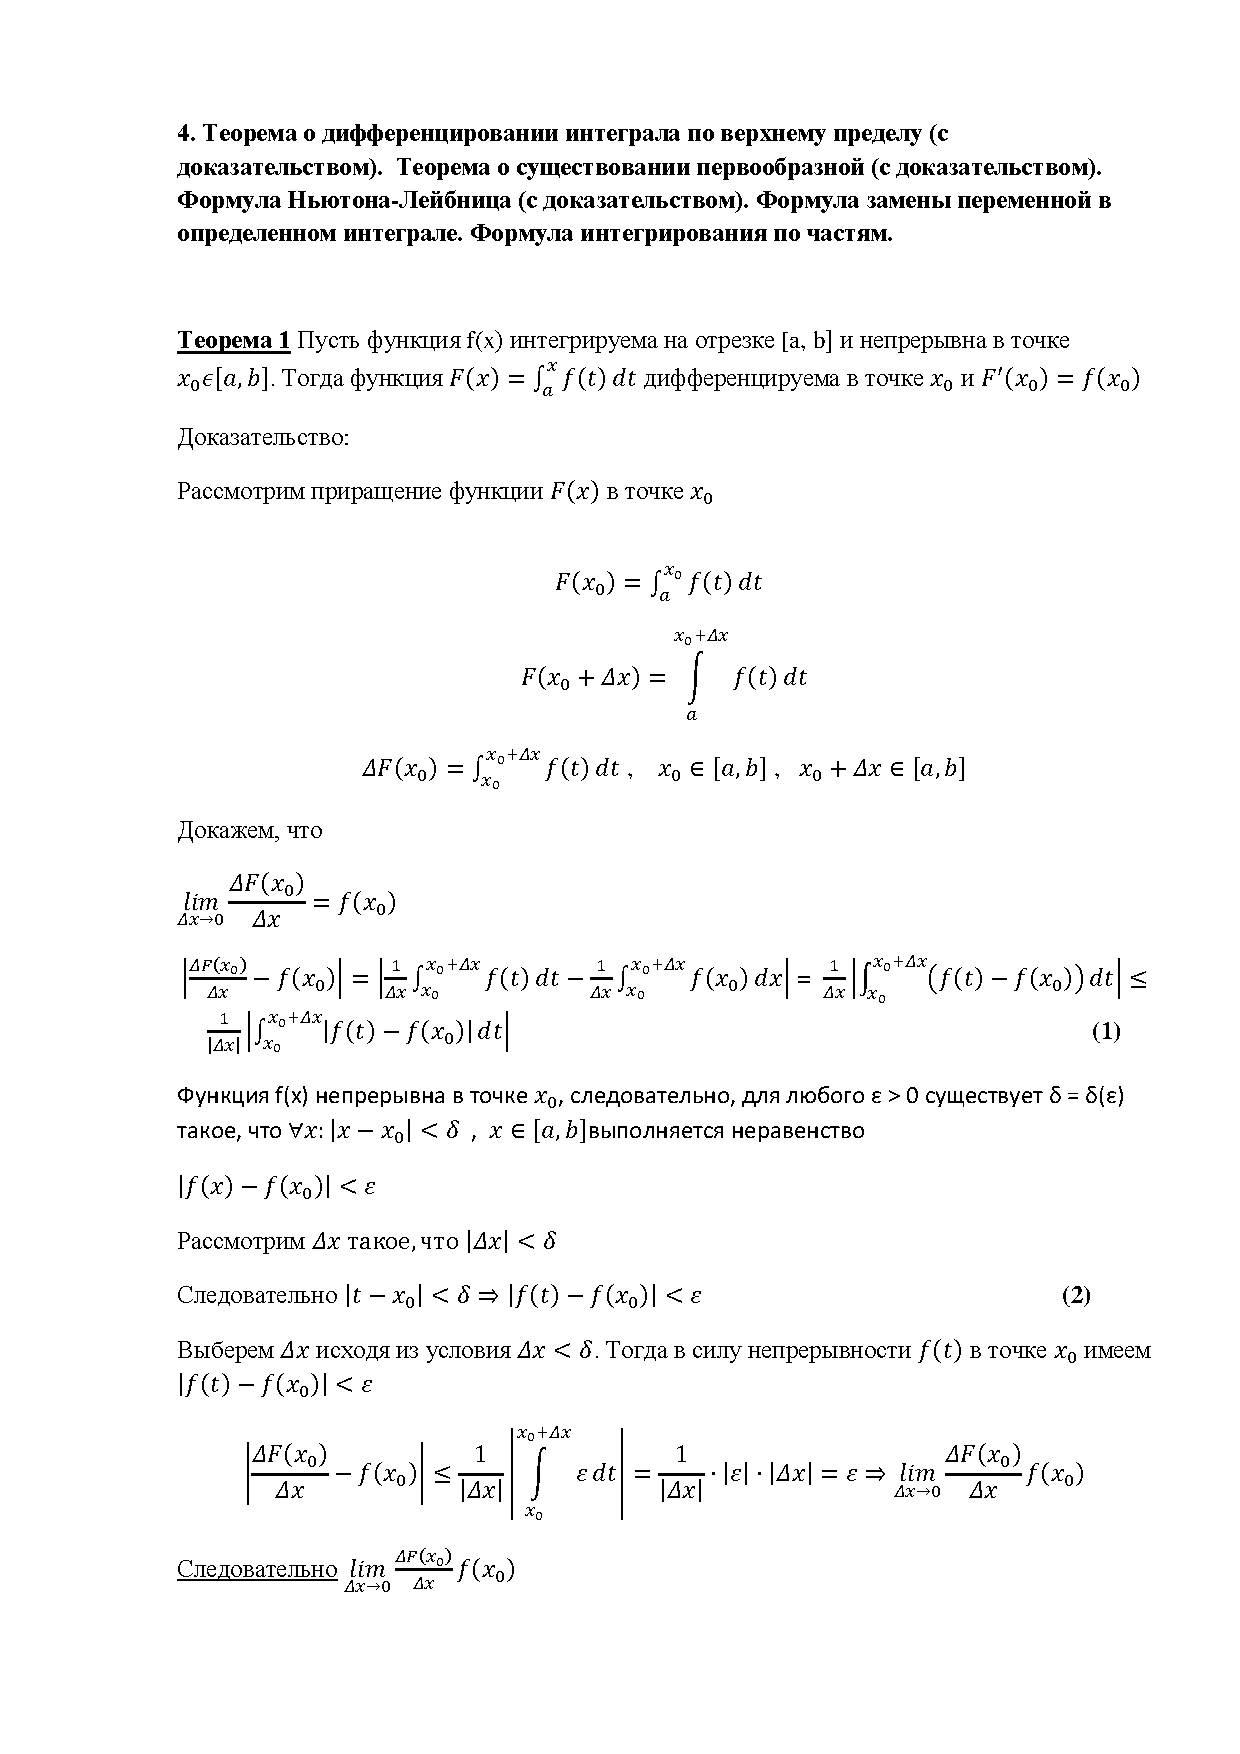
\includepdf[pages=-]{bilets/4.pdf}


\subsection{{\bfseries\sffamily DONE} Билет 5}
\label{sec:org3daad3c}
Определение несобственных интегралов.  Формула Ньютона-Лейбница и формула замены переменной для несобственных интегралов.
\href{bilets/5.pdf}{5}


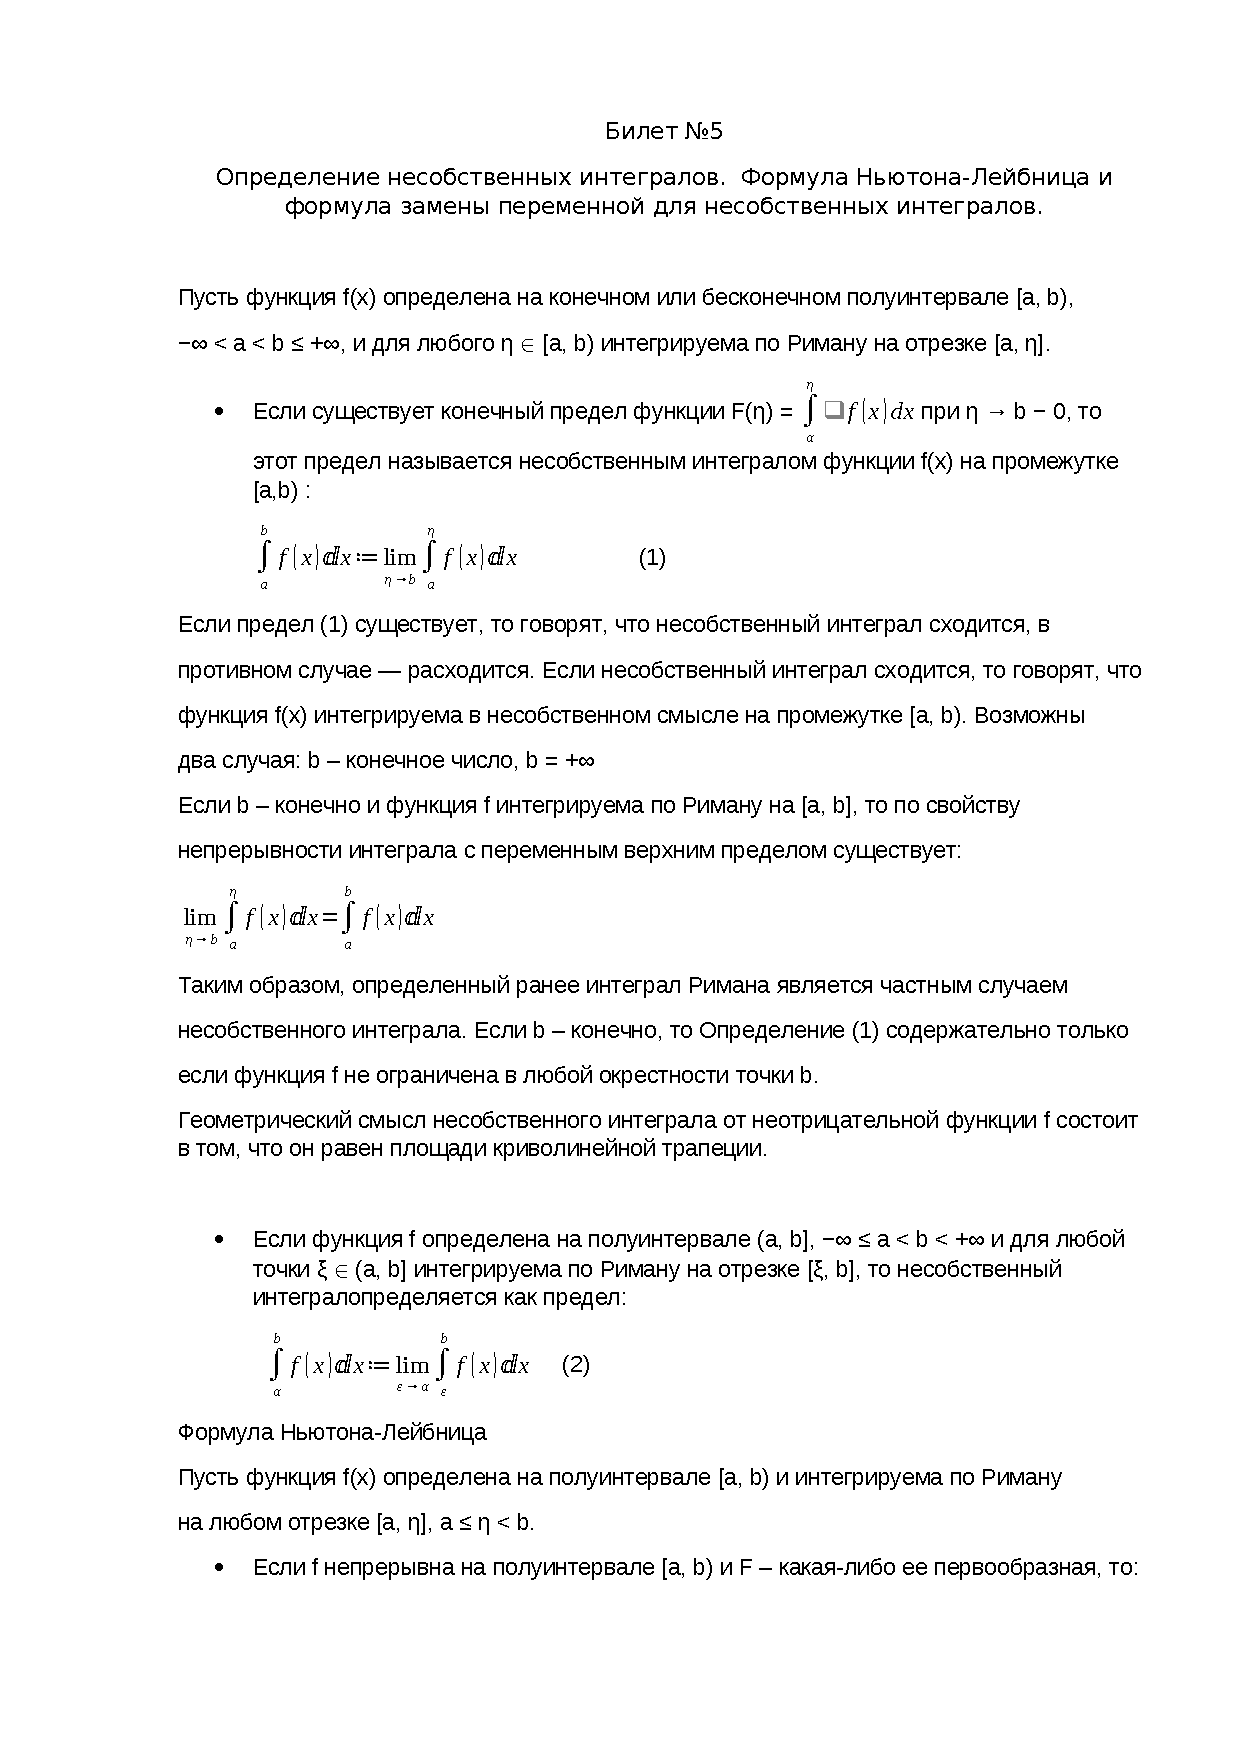
\includepdf[pages=-]{bilets/5.pdf}


\subsection{{\bfseries\sffamily DONE} Билет 6}
\label{sec:org0ff2b4d}
Несобственные интегралы от неотрицательных функций (лемма и признак сравнения). Критерий Коши сходимости интеграла (с доказательством). Абсолютно сходящиеся интегралы (определение и теорема о сходимости абсолютно сходящегося интеграла).
\href{bilets/6.pdf}{6}


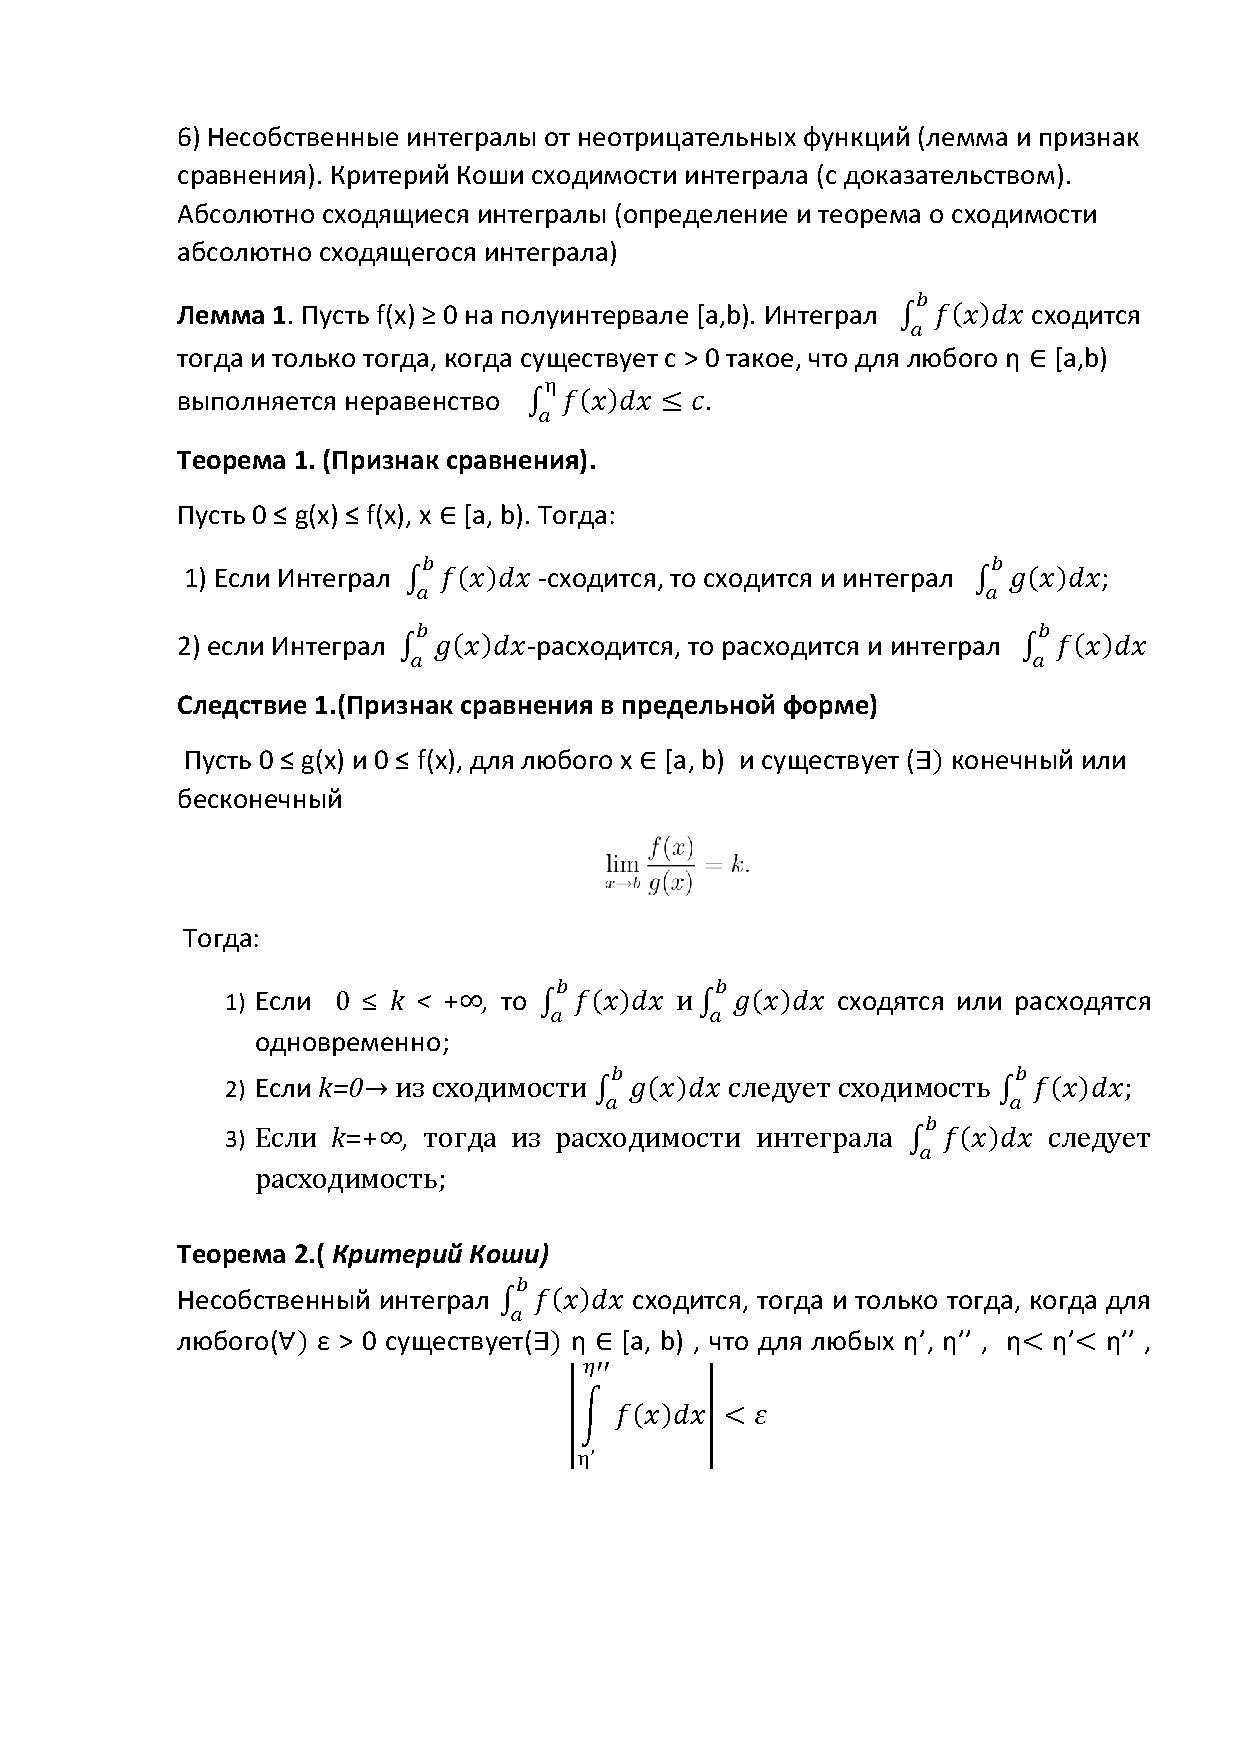
\includepdf[pages=-]{bilets/6.pdf}


\subsection{Билет 7}
\label{sec:org63a65b8}
Определение числового ряда. Необходимый признак сходимости ряда (с доказательством). Критерий Коши сходимости ряда (с доказательством). Ряды с неотрицательными членами (признак сравнения, интегральный признак Коши, радикальный признак Коши, признак Даламбера).

\subsection{{\bfseries\sffamily DONE} Билет 8}
\label{sec:orgcaa07c6}
Знакопеременные ряды (признак Лейбница). Абсолютно сходящиеся ряды (определение). Критерий Коши абсолютной сходимости ряда. Условно сходящиеся ряды (определение). Теорема Римана.
\href{bilets/8.pdf}{8}


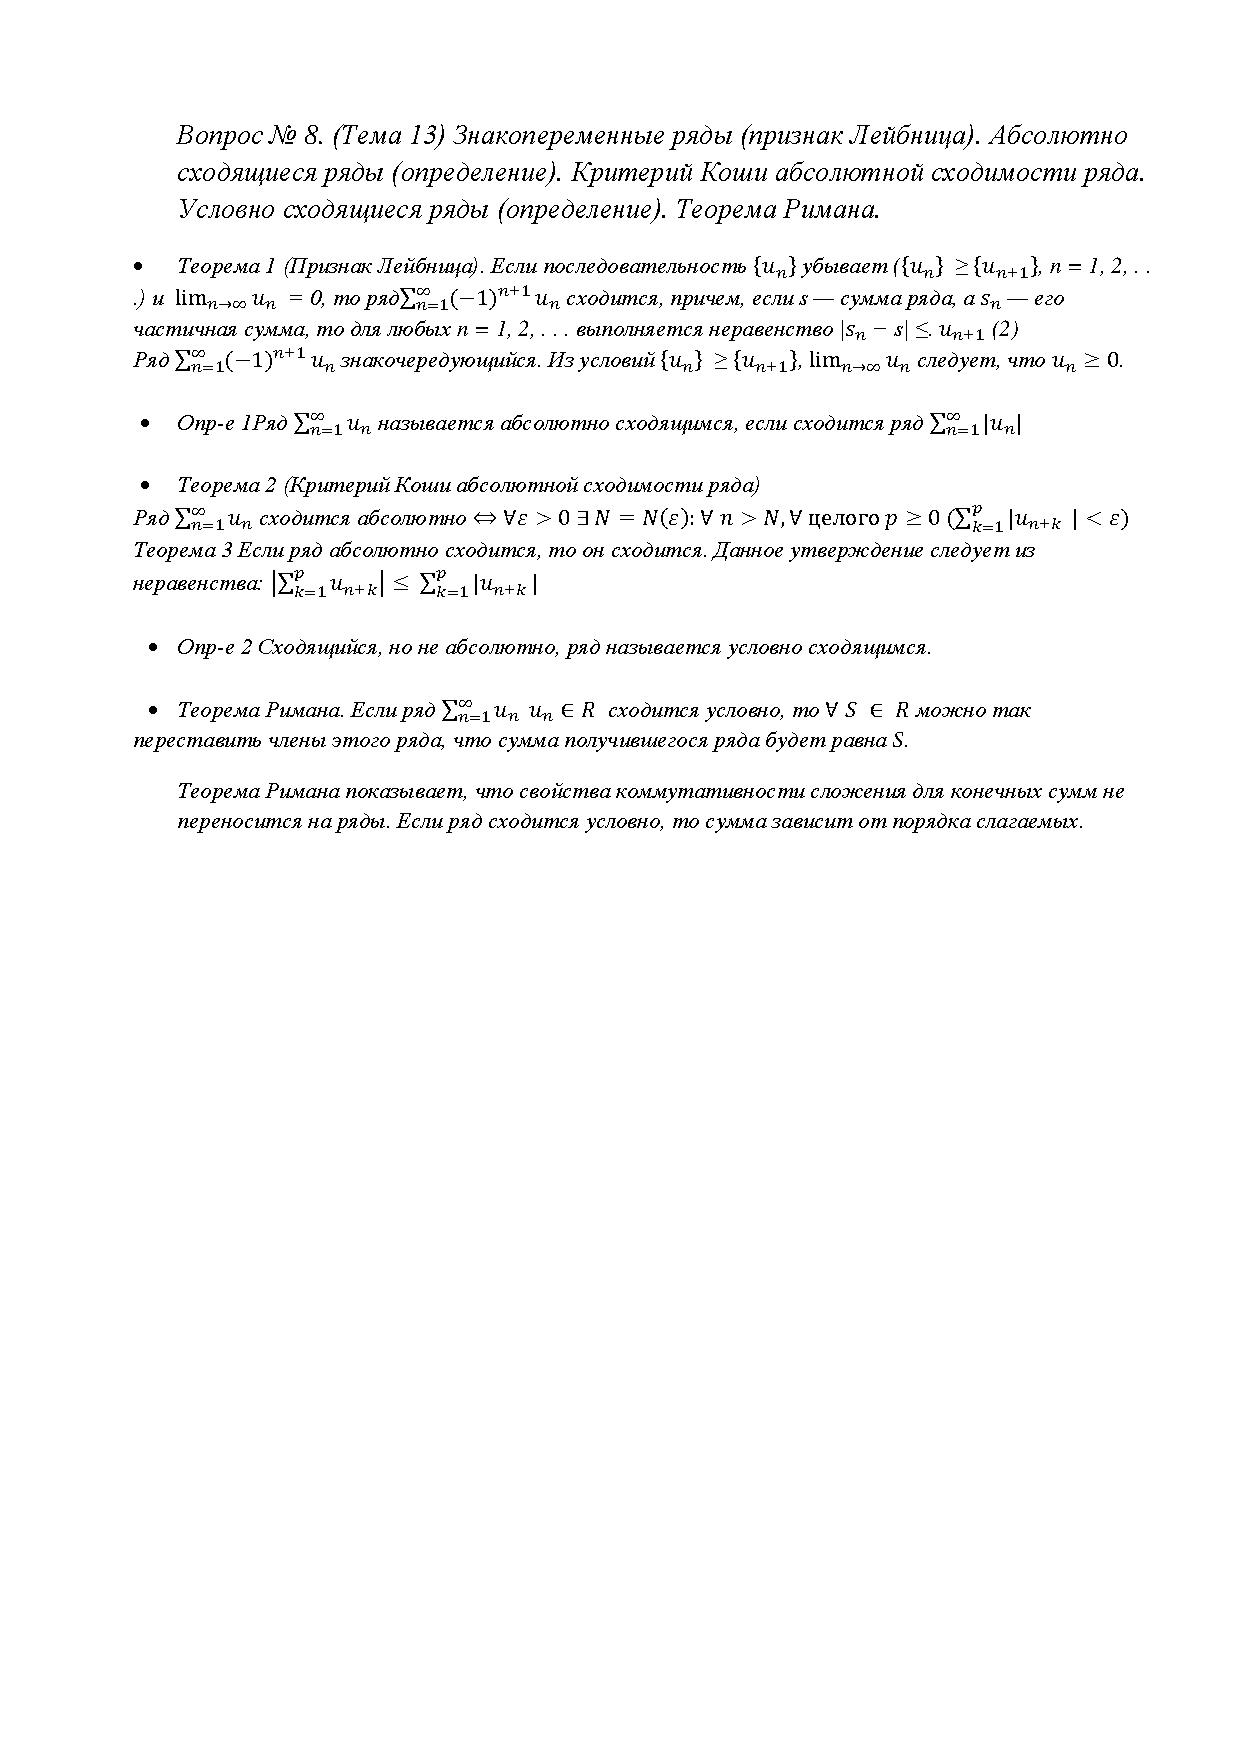
\includepdf[pages=-]{bilets/8.pdf}


\subsection{Билет 9}
\label{sec:org639ee08}
Функциональные последовательности  и ряды (определения, в том числе, ограниченная последовательность, сходящаяся последовательность, сходящийся ряд, абсолютно сходящийся ряд). Равномерная сходимость функциональной последовательности и функционального ряда (определение и пример). Критерии Коши равномерной сходимости функциональной последовательности (ряда). Признак Вейерштрасса.

\subsection{{\bfseries\sffamily DONE} Билет 10}
\label{sec:org48a448a}
Свойства равномерно сходящихся рядов (непрерывность суммы (с доказательством), интегрирование, дифференцирование).
\href{bilets/10.pdf}{10}


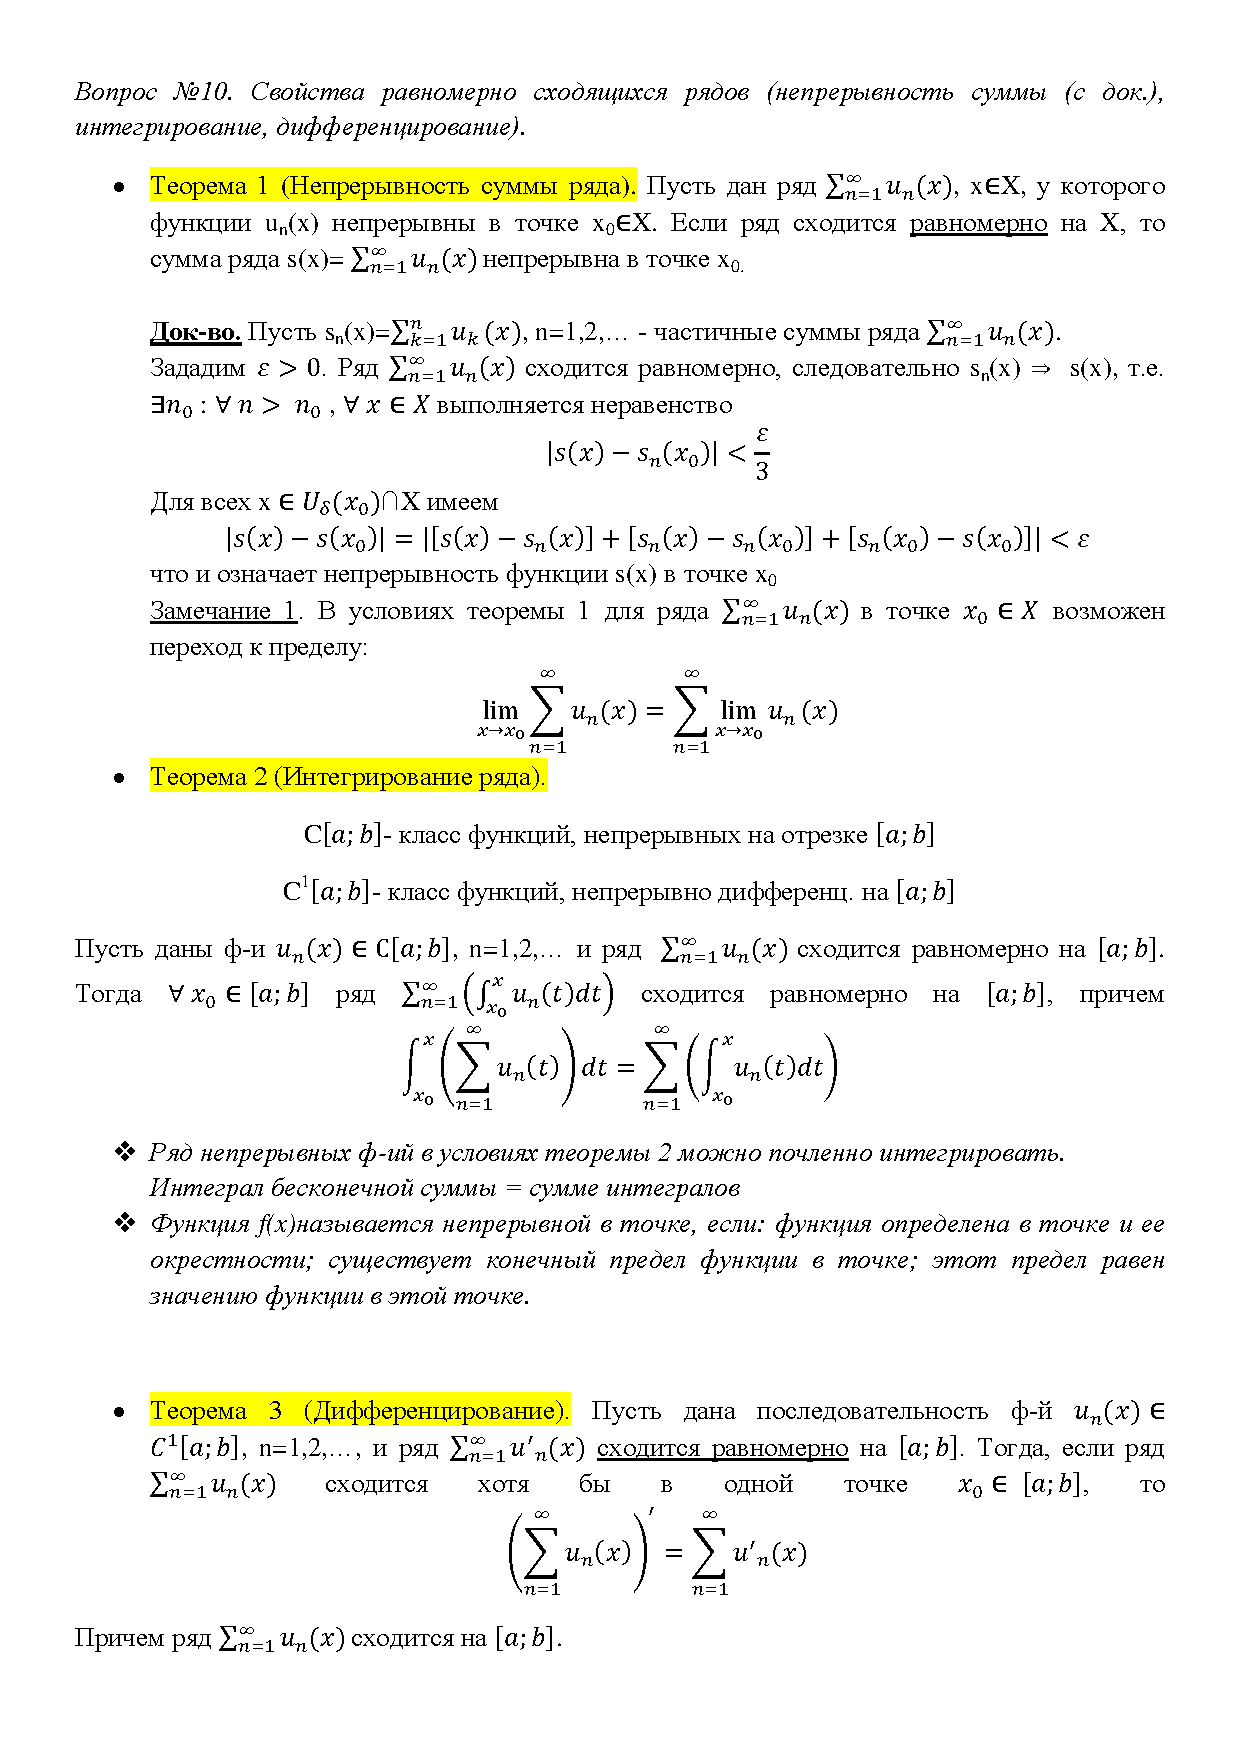
\includepdf[pages=-]{bilets/10.pdf}


\subsection{Билет 11}
\label{sec:org9efa93b}
Степенные ряды (определение). Первая теорема Абеля (с доказательством). Радиус и круг (интервал) сходимости степенного ряда (определения). Понятие аналитической функции (определение). Теорема о представлении аналитической функции рядом Тейлора.

\subsection{Билет 12}
\label{sec:org6f35079}
Определение n-мерного арифметического евклидова пространства. Определение n-мерного открытого шара. Предел последовательности в n-мерном пространстве, ограниченное множество  в n-мерном пространстве, окрестность бесконечно удалённой точки (определения).

\subsection{Билет 13}
\label{sec:org6b4f21c}
Внутренняя точка множества, открытое множество, точка прикосновения множества, предельная точка множества, замыкание множества, замкнутое множество, компактное множество, линейно связное множество, выпуклое множество, область (определения).
\end{document}
